\documentclass[a4paper, 12pt, twoside]{report}

\usepackage{physics, amsmath, amsfonts, systeme}
\usepackage{tcolorbox}
\usepackage{enumitem}
\usepackage{hyperref}
\usepackage{graphicx}
\hypersetup{
        colorlinks=true,
                linkcolor=black,
                urlcolor=blue,
}

\usepackage{geometry}
\geometry{
        top=2cm,
                bottom=2cm,
                left=2cm,
                right=3cm,
                headheight=17pt,
                includeheadfoot,
}

\usepackage{fancyhdr, lastpage}
\pagestyle{fancy}
\fancyhf{}
\lhead{Mettere icona GitHub}
\rhead{ Ottica }
\cfoot{Pagina \thepage\ di \pageref{LastPage}}
\renewcommand{\headrulewidth}{1.0pt}

\usepackage{etoolbox}
\patchcmd{\chapter}{\thispagestyle{plain}}{\thispagestyle{fancy}}{}{}

\title{Ottica}
\author{Pietro Garofalo}
\date{\today}


\begin{document}

\maketitle
\newpage
\tableofcontents
\chapter{Gli stati di polarizzazione}
In generale possiamo esprimere la luce come un campo elettrico 
\begin{align*}
    \va{E} = \va{E_{0}}\exp{i(\vb{k}\vb{r}-\omega t + \phi)}
\end{align*}
Il vettore $\va{E}$ è scomponibile in due componenti tra loro sempre ortogonali
\begin{tcolorbox}[colback=red!5!white,colframe=red!50!black,title=ATTENZIONE !]
        se la differenza di fase tra le due componenti $\va{E_{x}}$ ed $\va{E_{y}}$ si mantiene 
        costante si dice che la luce è \textbf{polarizzata}, se invece essa varia nel tempo 
        in modo casuale allora è \textbf{non polarizzata}, es la luce del sole.
\end{tcolorbox}
Semplicemente la polarizzazione ci dice come sono correlate le due componenti del campo elettrico, 
ve ne sono diverse, per esempio prendiamo una luce polarizzata circolarmente:
\begin{figure}[!h]
    \centering
    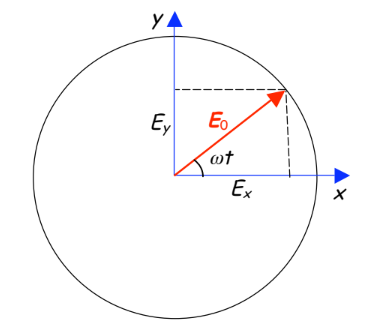
\includegraphics[scale=0.5]{polarizzazione/PolarizzazioneCirc} 
\end{figure}

ossia una luce che ha la compomente x massima quando quella y è nulla. 
\newpage
Possiamo rappresentarla nel seguente modo:
\begin{align*}
    \va{E} = \va{E}_{0x}\cos(kz-\omega t) + \va{E}_{0y}\sin(kz-\omega t)
\end{align*}
passando ora alla notazione complessa :
\begin{align*}
        \va{E} &= \va{E}_{0x}\exp{i(kz-\omega t)} + \va{E}_{0y}\exp{i(kz-\omega t)\pm \frac{\pi}{2}}\\[1em]
               &= \va{E}_{0x}\exp{i(kz-\omega t)} + \va{E}_{0y}i\exp{i(kz-\omega t)}
\end{align*}
dove non ho fatto altro che riscrivere il seno come il coseno più o meno $\frac{\pi}{2}$. \\
\section{Il vettore di Jones}
Dalla formula ricavata prima si nota subito che possiamo riscrivere l'onda come :
\begin{align*}
    \va{E} = \va{E}_{0}\va{J}\exp{i(kz-wt)}
\end{align*}
Dove il vettore $\va{J}$ rappresenta proprio la polarizzazione ed è definito come \textbf{vettore di Jones} che nel caso 
della polarizzazione circolare vale : 
\begin{align*}
        \va{J} = \begin{pmatrix} 1 \\ i \end{pmatrix}
\end{align*}
Tutte le polarizzazioni e i corrispondenti vettori di Jones li allego in figura
\begin{figure}[!h]
    \centering
    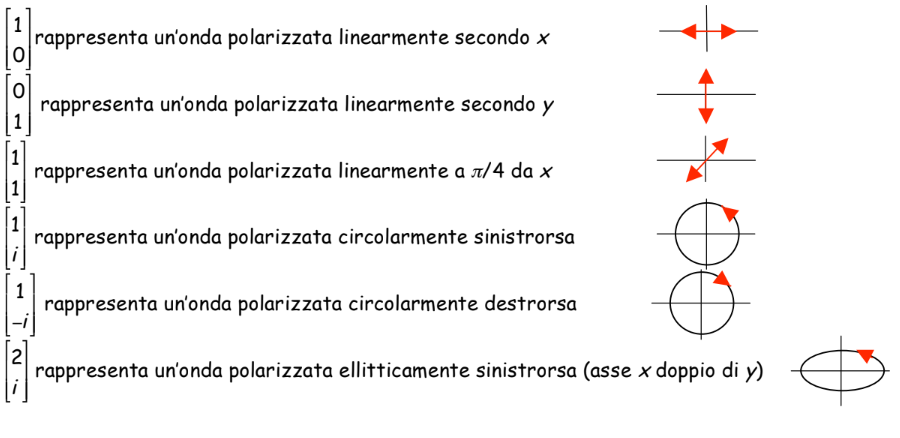
\includegraphics[scale=0.4]{polarizzazione/VettoriJones}
\end{figure}
In quest'ottica dunque gli effetti degli elementi ottici come per esempio le lamine $\lambda/4$ o $\lambda/2$, vengono 
rappresentati come \textbf{matrici di Jones}.
\newpage
\begin{figure}[!h]
    \centering
    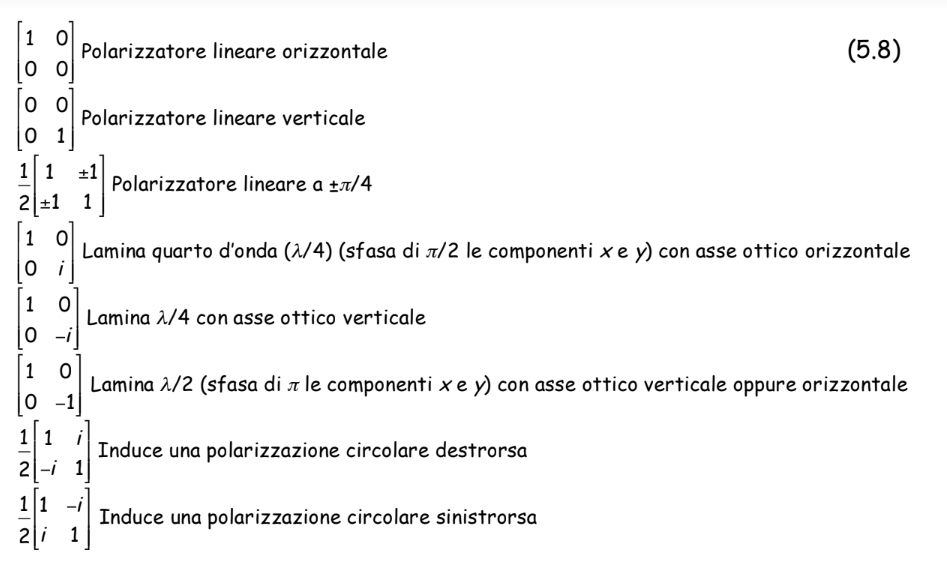
\includegraphics[scale=0.4]{polarizzazione/MatriciJones}
\end{figure}

Facciamo un esempio, prendiamo una luce polarizzata a 45 che passa attraverso una lamina $\lambda/4$:
\begin{align*}
    \begin{pmatrix} 1 & 0 \\ 0 & i\end{pmatrix}\begin{pmatrix}1\\1\end{pmatrix} = \begin{pmatrix}1\\i\end{pmatrix}
\end{align*}
si ottiene una luce polarizzata circolarmente.
Si possono ottenere inoltre gli effetti di altri elementi ottici ruotando quello originale.
Prendendo la matrice di rotazione : 
\begin{align*}
    R(\theta) = \begin{pmatrix}\cos{\theta} & \sin{\theta} \\ -\sin{\theta} & \cos{\theta} \end{pmatrix}
\end{align*}
allora la nuova matrice $\vb{T}^{\prime}$ si ottiene:
\begin{align*}
        \vb{T}^{\prime} = \vb{R}(\theta)\vb{T}\vb{R}(-\theta)
\end{align*}
\begin{tcolorbox}[colback=red!5!white,colframe=red!50!black,title=ATTENZIONE !]
Il fatto che se per esempio prendo un polaroid orizzontale e lo giro di 90 gradi ottendo un polaroid verticale 
funzione perchè gli elementi ottici hanno un asse preferenziale chiamato \textbf{asse ottico}
\end{tcolorbox}

\end{document}

